

%%
%%  This file was updated in April 2009 by J. Poole to be in line with Word tempaltes
%%
%%  Use \documentclass[boxit]{jacow}
%%  to draw a frame with the correct margins on the output.
%%
\documentclass{jacow}
%\documentclass{article}
%\usepackage{mathtools}
\usepackage{amsmath}
%%  for US letter paper layout
%%
\usepackage{graphicx}
\usepackage{booktabs}
%%
%%   VARIABLE HEIGHT FOR THE TITLE BOX (default 35mm)
%%

\setlength{\titleblockheight}{27mm}

\begin{document}
\title{The Development of Stochastic Processes in COSY Infinity}

\author{J. Kunz\thanks{jkunz@hawk.iit.edu}, P. Snopok, Illinois Institute of Technology, Chicago, IL 60616, USA\\
        M. Berz, K. Makino, Michigan State University, East Lansing, MI 48824, USA}

\maketitle

\begin{abstract}
COSY Infinity is an arbitrary-order beam dynamics simulation and analysis code. It can determine high-order transfer maps of combinations of particle optical elements of arbitrary field configurations. For precision modeling, design, and optimization of next-generation muon beam facilities, its features make it a very attractive code. Certain new features are being developed for inclusion in COSY to follow the distribution of charged particles through matter. To study in detail some of the properties of muons passing through material, the transfer map approach alone is not sufficient. The interplay of beam optics and atomic processes must be studied by a hybrid transfer map--Monte-Carlo approach in which transfer map methods describe the average behavior of the particles in the accelerator channel including energy loss, and Monte-Carlo methods are used to provide small corrections to the predictions of the transfer map accounting for the stochastic nature of scattering and straggling of particles. The advantage of the new approach is that it is very efficient in that the vast majority of the dynamics is represented by fast application of the high-order transfer map of an entire element and accumulated stochastic effects as well as possible particle decay. The gains in speed are expected to simplify the optimization of muon cooling channels which are usually very computationally demanding due to the need to repeatedly run large numbers of particles through large numbers of configurations. Progress on the development of the required algorithms is reported.
\end{abstract}

\section{INTRODUCTION}
Muon beams are tertiary production particles (protons to pions to muons) and high-intensity collection necessitates a large initial phase space volume. The resultant spray of muons must be collected, focused, and accelerated well within the muon lifetime (2.2~$\mu$s in the rest frame). The only technique fast enough to reduce the beam size within the muon lifetime is ionization cooling. Muons traverse a certain amount of material in order to lose energy in both longitudinal and transverse direction due to ionization. The energy is then restored in the longitudinal direction only, leading to an overall reduction in the transverse direction (cooling). In order to achieve cooling in the longitudinal direction, emittance exchange is used, usually involving wedge-shaped absorbers. For some applications, such as high-energy high-luminosity muon collider, cooling needs to be very aggressive: six-dimensional emittance reduction over six orders of magnitude is required to reach design goals.

In order to carefully simulate the effect of the absorbers on the beam, one needs to take into account both deterministic and stochastic effects in the ionization energy loss. The deterministic effects in the form of the Bethe-Bloch formula with various theoretical and experimental corrections fit well into the transfer map methods approach, where the effect of the lattice on the particles is evaluated first by producing the so-called transfer map, and then applied to a given initial distribution of particles. The arbitrary-order simulation code COSY Infinity \cite{COSY} is a key representative of the transfer map codes. COSY was chosen because of its built-in optomization tools, speed, its ability to produce high-order transfer maps, and its ability to control individual aberrations. 

However, to take into account the stochastic effects the transfer map paradigm needs to be augmented by either interfacing COSY with another code of choice (ICOOL,~\cite{ICOOL}) or implementing the corrections from stochastic effects directly into the fabric of COSY. Some of the fundamental ideas of the process were presented in~\cite{errede} in application to the quadrupole cooling channels, but the approximations used were fairly basic. ICOOL is a code written specifically to study the ionization cooling of muon beams. The discussion of the selection and interfacing process can be found in~\cite{napac13}. The long-term plan is to incorporate multiple scattering and energy straggling models into COSY thus avoiding any interfacing with an external code.

%COSY Infinity is a beamline simulations tool used in the design, analysis, and optomization of particle accelerators~\cite{COSY-ref}. To do this, COSY uses the transfer map approach, which evaluates the overall effect of a system on a beam of particles  using differential algebra (involving multivariate Taylor polynomials up to arbitrary order). While a transfer map is technically not a nonlinear matrix, it is sometimes helpful to think of them as one in the same. Along with the evaluation of particles through a lattice, COSY also has a plethora of analysis and optomization tools, including (but not limited to) lattice aberration and correction tools, support for Twiss parameters, support for tunes and nonlinear tune shifts, built-in optimizers (for lattice design), and spin tracking. \par

%COSY is particularly advantageous to use when considering the efficient use of computational time. This is due to the transfer map methods that COSY employs. Given some initial phase space vector
%\begin{equation}
%\mathbf{Z}=
%\begin{pmatrix}
%x\\ y\\ l=k(t-t_0)\\a=p_x/p_0\\b=p_y/p_0\\  \delta = (E-E_0)/E_0
%\end{pmatrix}
%\end{equation}
%where the so-called particle optical coordinates are transverse positions ($x, y$), time-of-flight in units of length ($l$), transverse angles w.r.t. the reference particle ($a, b$), and kinetic energy deviations w.r.t. the reference particle ($\delta$), and the $0$ subscript in the definitions denotes the reference particle's properties, the transfer map $\mathcal{M}$ will uniquely predict the time evolution of $\mathbf{Z}$. This is because most beam elements follow Maxwell's equations, which yield unique solutions that are dependent on initial conditions. Mathematically, this relationship is $\mathbf{Z}(s)=\mathcal{M}(s_0 , s)*\mathbf{Z}(s_0)$. Here, the independent variable $s$ is understood as the reference orbit (the zero point of a beam of particles in some comoving reference frame --see Figure 2). Now, the composition of two maps yeilds another map: $\mathcal{M}(s_1 , s_2)\times \mathcal{M}(s_0 , s_1) = \mathcal{M}(s_0 , s_2)$. Therefore, it is possible to "cut out" the middle part $s_1$. Since each physical lattice corresponds to some transfer map, it is possible to construct a single map that represents many individual lattices. Computationally this is advantageous because once calculated, it is much faster to apply a solitary transfer map to a distribution of particles than to simulate that same distribution through many meters of lattices.
%\par

\section{Stochastic Effects}

COSY supports a large variety of lattice elements such as magnetic and electric multipoles (with or without fringe fields), homogeneous and inhomogeneous bending elements, Wien filters, wigglers and undulators, cavities, cylindrical electromagnetic lenses, general particle optical elements, and \emph{deterministic} polynomial absorbers of arbitrary order, with the last element being of particular interest for the cooling simulations.

%\begin{figure}[h!]
%\centering
%\includegraphics*[width=70mm]{C:/Users/kunzj_000/Desktop/dissertation_mats/figure2}
%\caption{The reference orbit.}
%\end{figure}

The term ``deterministic'' is deliberately emphasized, since the polynomial absorber acts like a drift with Bethe-Bloch energy loss. The advantage of this is that the user must only specify six material parameters in order for COSY to calculate this energy loss; in particular, the user must specify the $Z$ number, $A$ number, density, ionization potential, density correction parameter, and shell correction parameter.

However, this element only takes into account deterministic effects (effects which produce the same final result the same initial conditions), not stochastic effects (pseudo-random effects such as multiple scattering and straggling).

Equation~\eqref{emittance} describes the evolution of the normalized transverse emittance along the cooling channel, where $\epsilon_n$ is the normalized emittance, $z$ is the path length, $E_\mu$ is the muon beam energy, $\beta = v/c$, $L_R$ is the radiation length of the absorber material, $\beta_\perp$ is the betatron function, and $E_s$ is the characteristic scattering energy:

\begin{equation}
\frac{d\epsilon_n }{dz} \approx -\frac{1}{\beta^2} \left< \frac{dE_\mu}{dz} \right> \frac{\epsilon_n}{E_\mu} + \frac{1}{\beta^3} \frac{\beta_\perp E_s ^2}{2E_\mu mc^2 L_R}.
\label{emittance}
\end{equation}

Here, two competing effects can be seen: the first term is the cooling (reduction of beam size) component from ionization energy loss and the second term is the heating (increase of beam size) term from multiple scattering. This highlights the importance of the stochastic terms, as the only deterministic term is the expected (Bethe-Bloch) energy loss, $\left< dE_\mu/dz \right>$ and there is no equilibrium emittance which is unrealistic.

Stochastic effects do not fit well into the transfer map paradigm and require special treatment. To illustrate this, start with a number of particles with identical initial coordinates. As seen in Figure~\ref{fig:mult_scattering}, these initially indistinguishable particles follow different paths in material due to the random nature of multiple scattering. Therefore, it is not possible to construct a traditional transfer map that represents the absorber. This would require uniquely relating the coordinates after the absorber to the coordinates before the absorber.

\begin{figure}[htb]
\centering
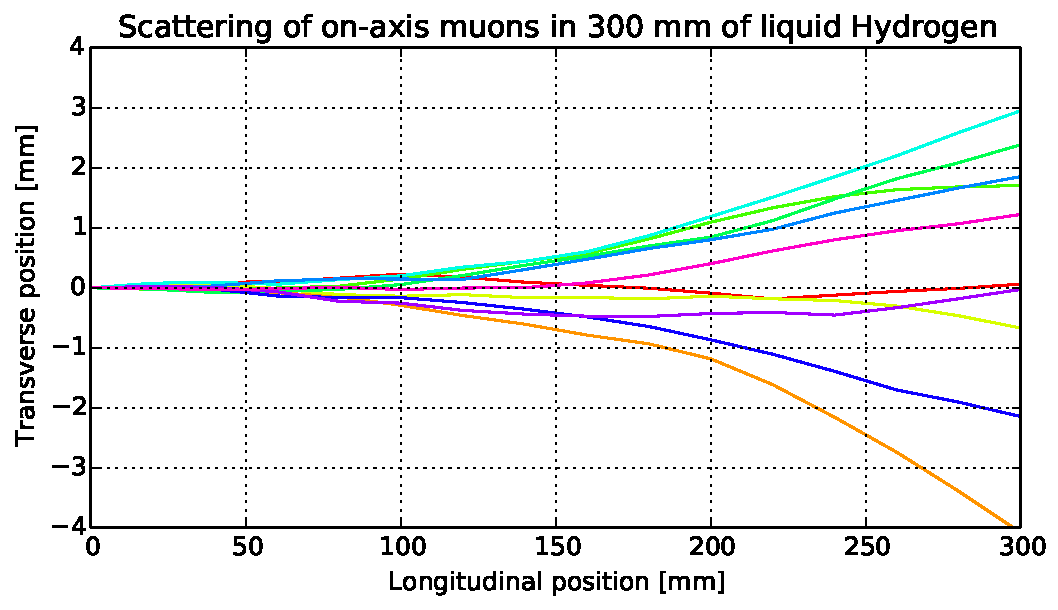
\includegraphics[width=0.49\textwidth]{figures/p10tr.pdf}
\caption{Possible scatterings of a particle through matter. Due to the random nature of multiple scattering, a particle may scatter at a variety of angles when traversing matter.}
\label{fig:mult_scattering}
\end{figure}

%To further stress the importance of stochastic effects as a part of realistic simulations, COSY was compared to another program called ICOOL [2]. This was done by the simulation of a flat 32 cm liquid hydrogen absorber proceeded and followed by 10 cm drifts. ICOOL is a particle-by-particle propagation code written for the study of ionization cooling of muon beams. Therefore, the discrepancy between these two codes is largely due to stochastic effects. The results of this simulation are found in Table 1. Here, it is clear that while the longitudinal coordinates appear to agree well, the transverse coordinates do not. Moreover, the large discrepancy between the X and Y percent disagreements is likely because the initial distributions were randomly centered about (X, Px, Y, Py) = (0, 0, 0, 0).

%\begin{table}[htb]
%   \centering
%   \caption{Results of a comparison simulation between COSY and ICOOL. The simulation was of a 32 cm flat liquid hydrogen absorber proceeded and followed by 10 cm drifts. The discrepancy between the two codes is understood as whether or not the code consideres stochastic effects.}
%   \begin{tabular}{lcccc}
%       \toprule
%			 \textbf{}            & \textbf{Initial} 	& \textbf{Final (COSY)} & \textbf{Final (ICOOL)} 	& \textbf{\% Disagreement (w.r.t. ICOOL)} \\ 
%          $ X (mm)$      &0.001572 &-1.862 &-1.756 &6.04\\
%	$\sigma_X (mm)$&0.967&26.617&27.150&1.96\\
%	$P_X (MeV)$&-3.584&-0.6612&-0.6120&8.04\\
%	$\sigma_{P_X} (MeV)$&51.151&9.498&9.899&4.05\\
%	$Y (mm)$&0.018172&-0.8227&-1.055&22.02\\
%	$\sigma_Y (mm)$&1.035&26.080&26.050&0.12\\
%	$P_Y (MeV)$&-1.617&-.373&-0.4490&31.56\\
%	$\sigma_{P_Y} (MeV)$&50.234&9.331&9.423&0.98\\
%	$P (MeV)$&200.228&189.173&189.114&0.03\\
%	$\sigma_P (MeV)$&19.883&20.534&20.528&0.03\\
%       \bottomrule
%   \end{tabular}
%   \label{l2ea4-t1}
%\end{table}

%However, here it is important to note that the standard deviation of the longitudinal coordinates may not be well-defined, as the energy loss of particles through a material follows a Landau distribution, not Gaussian. This was not accounted for until recently, and as such the standard deviation was used in spite of this fact. \par

%\section{MOTIVATION}
%
%A prime example of why matter-dominated lattices are relevant comes from the prospect of a Muon Collider. While the Large Hadron Collider is roughly 27 km in circumference and the next proposed hadron collider could be up to 50 km, a high energy muon collider ($\sqrt{s}=$ 6.0 TeV) could be built on the existing Fermilab site (roughly 6 km in circumference) [8]. Additionally, a muon collider could serve as a Higgs factory ($\sqrt{s}=$126 GeV), with possible new physics via the observation of Higgs to lepton coupling. Moreover, as muon branching fractions are 100\% neutrino-antineutrino, there are obvious advantages of a muon-sourced neutrino beam. \par
%
%However, muon-based facilities are not without their challenges. Muons are unstable particles, and have a rest-frame lifetime of 2.2 $\mu$s. Therefore, beam cooling techniques which are used for protons and electrons cannot be used, as they are too slow. Synthetic muon creation comes from the collision of protons on a fixed target. The resultant spray of particles largely contains kaons (which decay primarily into pions and muons), pions (which decay primarily into muons), and rogue protons. Therefore, high-intensity collection necessitates a large initial phase space volume. The resultant cloud of muons must be collected, focused, and accelerated well within the muon lifetime (2.2 $\mu$s). Due to the short-lived nature of the muon, novel beam cooling (beam size reduction) techniques have been explored and 6D ionization cooling in particular has been shown to work quite well [5,6]. Muons traverse a certain amount of material in order to lose energy in both longitudinal and transverse direction due to ionization. The energy is then manually restored in the longitudinal direction only, leading to an overall reduction in the transverse direction (cooling). In order to achieve cooling in the longitudinal direction, emittance exchange is used, usually involving wedge-shaped absorbers. The result of such an emittance exchange scheme can be seen in Figure 4 [7]. \par
%
%\begin{figure}[h!]
%\centering
%\includegraphics*[width=70mm]{C:/Users/kunzj_000/Desktop/dissertation_mats/figure4}
%\caption{Emittance exchange.}
%\end{figure}


\section{STOCHASTIC PROCESSES IN COSY AND SIMULATION RESULTS}
It has been shown that the inclusion of stochastic processes into COSY Infinity would be both necessary for realistic simulation and relevant to future experiments. The ultimate goal of this work is to add new tools to COSY which would accurately take into account stochastic effects without compromising COSY's computational efficiency. 

The first method proposed was to interface COSY with an external code (ICOOL or G4beamline), so that part of that code is invoked whenever an absorber is encountered in the way of the beam. Unfortunately, this method suffers from the overhead of initializing external code and passing particle distributions back and forth. This issue could be mitigated partially by letting COSY handle the average energy loss in the absorber, and incorporating the parts of the external code handling multiple scattering and energy straggling directly into COSY. However, this method involves splitting the absorber into thin segments for precision considerations, thus affecting the speed of the simulation. That said, the preliminary results using the latter method were encouraging, and we may return to that study at some point.

The algorithm that is currently under active study, applies a perturbative kick to each particle at the end of the absorber, thereby emulating stochastic effects. The strength and variety of this kick depends on two parameters: the initial energy of the particle and the length of absorber that the particle traverses (equivalently, the average amount of energy lost within the material). This can be done because the particle's coordinates follow predictable patterns when it travels through matter, as can be seen in Figures~\ref{fig:scattering} and~\ref{fig:straggling} (raw data generated by ICOOL).

\begin{figure}[htb]
\centering
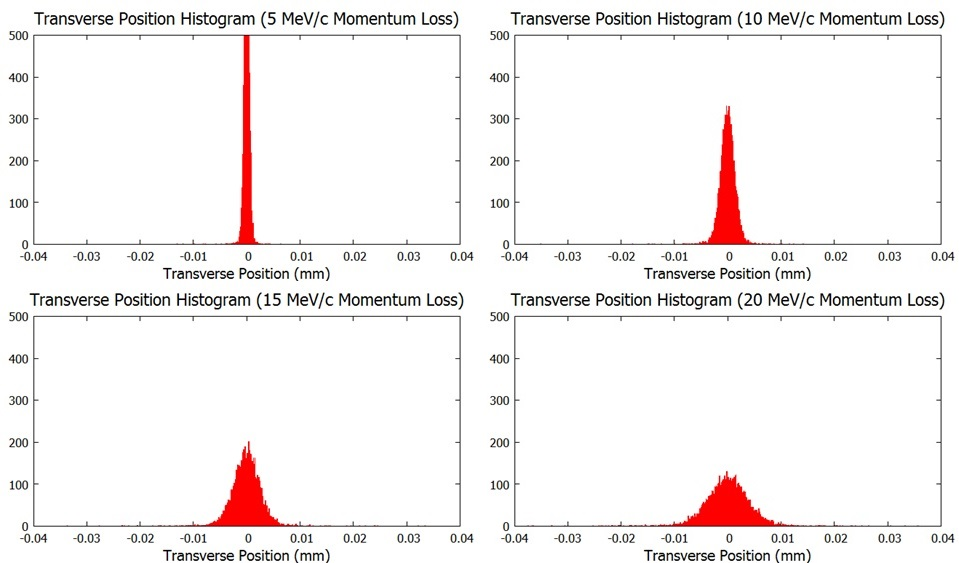
\includegraphics[width=0.49\textwidth]{figures/scattering.jpg}
\caption{Transverse position histograms for four different absorber lengths corresponding to 5, 10, 15, and 20 MeV$/c$ momentum loss. The initial distribution was a pencil beam of 10,000 muons with an initial momentum of 200 MeV$/c$.}
\label{fig:scattering}
\end{figure}

\begin{figure}[htb]
\centering
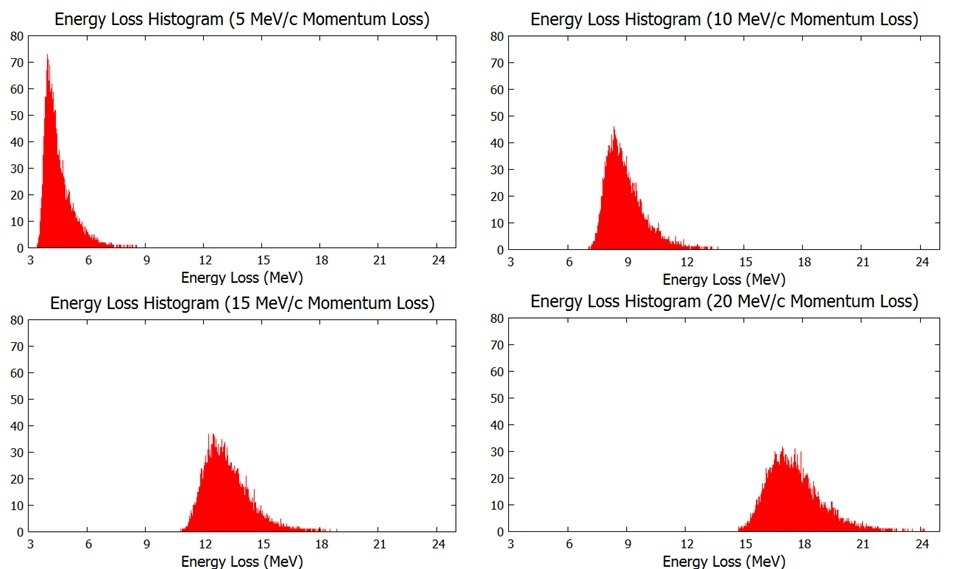
\includegraphics[width=0.49\textwidth]{figures/straggling.jpg}
\caption{Energy loss histograms for four different absorber lengths corresponding to 5, 10, 15, and 20 MeV$/c$ momentum loss. The initial distribution was a pencil beam of 10,000 muons with an initial momentum of 200 MeV$/c$.}
\label{fig:straggling}
\end{figure}

When COSY applies the effects of an absorber onto a distribution of particles, two events occur: the transfer map method accounts for average energy loss following the Bethe--Bloch curve, and the new algorithm applies a random kick to each particle's coordinates. For example, Figure~\ref{fig:scattering} shows that the correction to the transverse position of a particle is nearly Gaussian. The mean of the distribution is zero, while the standard deviation $\sigma$ varies depending on the path length through the absorber, which COSY conveniently already calculates as part of the transfer map method. Therefore, it is possible to represent $\sigma$ as a function of initial energy and absorber length. For this reason, the method and its collective subroutines have been referred to as the ``functional method''. Figure~\ref{fig:functional} shows an example plot of $\sigma$ versus average energy loss (equivalently, absorber length) for a pencil beam of 10,000 muons with an initial momentum of 200 MeV$/c$. The functional method allows for a relatively compact storage of functional dependencies as compared to storing huge tables of numbers corresponding to each and every combination of absorber length and material, and initial energy of the particle. The key assumption is that the stochastic effects can be represented by a known random distribution with relatively few parameters. At the moment we use Gaussian approximation for multiple scattering, potentially adding Rutherford-like tails; and Landau distribution for energy straggling in thin absorbers or a convolution of Landau and Gaussian for thicker absorbers.

\begin{figure}[htf]
\centering
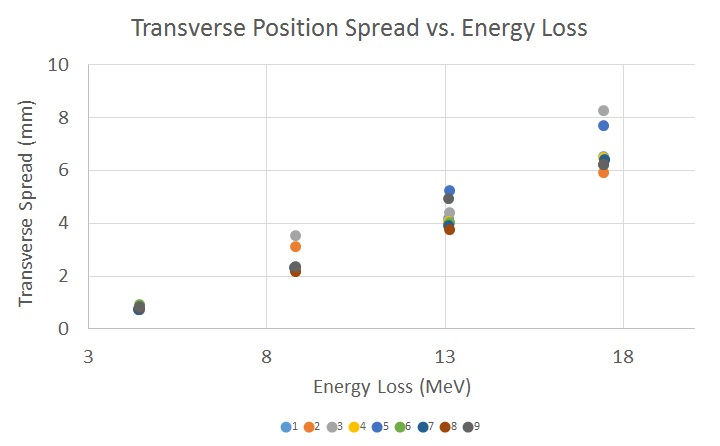
\includegraphics[width=0.49\textwidth]{figures/functional.jpg}
\caption{Scattering distribution $\sigma$ versus average energy loss in the absorber.}
\label{fig:functional}
\end{figure}

To test this method, a one-dimensional Gaussian distribution of 10,000 muons with parameters $\sigma_x=10$~mm, $\sigma_{p_x}=10$ keV and initial momenta of 200 MeV$/c$ ($\sigma_{p_z} = 0$) was generated and simulated through a 90$^\circ$ liquid hydrogen wedge absorber with an on-axis thickness of 32 cm. The absorber was preceded and followed by 10-cm drifts. This ensured that each particle went through a different amount of material. These conditions were simulated in COSY without the functional method and compared with COSY augmented with the functional method and an independent ICOOL run. The results can be found in Table~\ref{tab:comparison}.

\begin{table}[hbt]
   \centering
   \caption{Baseline COSY vs Functional COSY vs ICOOL.}
   \begin{tabular}{lccc}
       \toprule
	\textbf{}& \textbf{Baseline} & \textbf{Functional}& \textbf{ICOOL} \\ 
	\textbf{}& \textbf{COSY} & \textbf{COSY}& \textbf{} \\ 
          $ \sigma_X (mm)$&18.96&19.05&19.04\\
	$\sigma_Y (mm)$&19.00&19.06&19.10\\
	\bottomrule
   \end{tabular}
   \label{tab:comparison}
\end{table}

\section{SUMMARY}
New methods are being explored and implemented in COSY to allow for the simulation of stochastic processes in matter-dominated muon accelerators. The so-called functional method is proposed and currently under active study, work continues along multiple directions: find better fits describing multiple scattering and energy straggling for a variety of absorber thicknesses and muon initial energies; deduce the effects from first principles in order not to rely on any particular external code; and compare the results with experimental data.

To this end, steady progress is being made, and it is anticipated that COSY will make use of the functional method for the efficient and robust simulation of particles through matter.

\begin{thebibliography}{9}   % Use for  1-9  references
\bibitem{COSY} 
COSY Infinity, \url{http://www.bt.pa.msu.edu/index_cosy.htm}
\bibitem{ICOOL} 
ICOOL, \url{https://pubweb.bnl.gov/~fernow/icool/readme.html}
\bibitem{errede}
D. Errede \emph{et al.} Stochastic processes in muon ionization cooling, \emph {NIM A,} 519 (2004) 466--471.
\bibitem{napac13}
P. Snopok, J. Kunz. Progress of the matter-dominated muon accelerator lattice simulation tools development for COSY Infinity. Proc. of NA-PAC'13, MOPBA10, 2013.
%\bibitem{Kim-ref}
%E.S. Kim, M. Yoon, Design of Transverse Muon-Cooling Channels for a Neutrino Factory, Japan Journal of Applied Physics Vol. 40, pp. 401-406, 2001, \texttt{http://www-mucool.fnal.gov/mcnotes/public/pdf/muc0225/muc0225.pdf}.
%\bibitem{Bravar-ref}
%U. Bravar et al., MICE: the Muon Ionization Cooling Experiment, Proceedings of the DPF-2011 Conference, 2011, \texttt{http://arxiv.org/ftp/arxiv/papers/1110/1110.1813.pdf}.
%\bibitem{MuScat-ref}
%MuScat Collaboration, The scattering of muons in  low Z materials, 2005, \texttt{http://arxiv.org/abs/hep-ex/0512005}.
%\bibitem{Fermilab-ref}
%Fermilab, A Feasibility Study of a Neutrino Source Based on a Muon Storage Ring, edited by N. Holtkamp and D. Finley, 2000.
%\bibitem{Palmer-ref}
%M. Palmer, The R\&D Program For A Future Muon Collider, 2013, \texttt{http://accelconf.web.cern.ch/AccelConf/pac2013/talks/moyaa2\_talk.pdf}.
%\bibitem{Eichten-ref}
%E. Eichten, Physics at a Muon Collider Higgs Factory, 2013, \texttt{https://hepconf.physics.ucla.edu/higgs2013/talks/eichten.pdf}.

\end{thebibliography}
\mbox{}
\end{document}
